%%%%%%%%%%%%%%%%%%%%%%%%%%%%%%%%%%%%%%%%%
% fphw Assignment
% LaTeX Template
% Version 1.0 (27/04/2019)
%
% This template originates from:
% https://www.LaTeXTemplates.com
%
% Authors:
% Class by Felipe Portales-Oliva (f.portales.oliva@gmail.com) with template 
% content and modifications by Vel (vel@LaTeXTemplates.com)
%
% Template (this file) License:
% CC BY-NC-SA 3.0 (http://creativecommons.org/licenses/by-nc-sa/3.0/)
%
%%%%%%%%%%%%%%%%%%%%%%%%%%%%%%%%%%%%%%%%%

%----------------------------------------------------------------------------------------
%	PACKAGES AND OTHER DOCUMENT CONFIGURATIONS
%----------------------------------------------------------------------------------------

\documentclass[
	12pt, % Default font size, values between 10pt-12pt are allowed
	%letterpaper, % Uncomment for US letter paper size
	%spanish, % Uncomment for Spanish
]{fphw}

% Template-specific packages
\usepackage[utf8]{inputenc} % Required for inputting international characters
\usepackage[T1]{fontenc} % Output font encoding for international characters
\usepackage{mathpazo} % Use the Palatino font
\usepackage{setspace}

\usepackage{graphicx} % Required for including images

\usepackage{booktabs} % Required for better horizontal rules in tables

\usepackage{listings} % Required for insertion of code

\usepackage{enumerate} % To modify the enumerate environment

\usepackage{parskip}% http://ctan.org/pkg/parskip

\usepackage{amsmath}

\usepackage{caption}

%----------------------------------------------------------------------------------------
%	ASSIGNMENT INFORMATION
%----------------------------------------------------------------------------------------

\title{AULA 7 - Implementação da programação modular} % Assignment title

\author{AVC, JPP, PC} % Student name

\date{} % Due date

\institute{Pontifícia Universidade Católica do Rio de Janeiro \\ Departamento de Informática} % Institute or school name

\class{Programação Modular (INF1301)} % Course or class name

\professor{Flavio Bevilacqua} % Professor or teacher in charge of the assignment

%----------------------------------------------------------------------------------------

\begin{document}

\maketitle % Output the assignment title, created automatically using the information in the custom commands above

%----------------------------------------------------------------------------------------
%	ASSIGNMENT CONTENT
%----------------------------------------------------------------------------------------
\begin{doublespace}

    \begin{enumerate}

        \item Espaço de dados

              Áreas de armazenamento:

              \begin{itemize}

                  \item Possuem nome (um ou mais).
                  \item Possuem tamanho.
                  \item Alocados em um meio.

              \end{itemize}

              Exemplos:

              A[j] $\implies$ j-ésima posição do vetor A.

              *ptAux $\implies$ espaço referenciado por ptAux.

              ptAux $\implies$ espaço que contém um endereço de memória.

              ptElemTabSimb *ObterElemTabSimb(char *ptSimbolo)

              (*ObterElemTabSimb(char *ptSimb)).Id $\implies$ campo Id da estrutura apontada pelo ponteiro retornado pela função.

              ObterElemTabSimb(char *ptSimb)$\rightarrow$Id $\implies$ o mesmo que o anterior.

        \item Tipos de dados

              \textbf{define:}

              \begin{itemize}

                  \item Organização
                  \item Codificação

                        Data: AAAAMMDD
                        CPF: xxxxxxxxx-xx

                  \item tamanho
                  \item Conjunto de valores permitidos

              \end{itemize}

              \textbf{OBS: Tipos de tipo}

              \begin{itemize}

                  \item Computacional. Ex: int, char*, float
                  \item Tipos abstratos de dados. Ex: estrutura encapsulada que só é conhecida pelos clientes através de funções de acesso.
                  \item Tipos básicos de usuário (typedef, enum, union, struct).

              \end{itemize}

              \textbf{typedef:}

              Exemplo:

              typedef float tpVeloc;

              typedef float tpTempo;

              tpVeloc veloc;

              tpTempo tempo;

        \item Declaração e definição de elementos

              Declarar é vincular a um tipo. Typecast não é declaração.

              Definir é alocar um espaço na memória e vincular um espaço a um nome (binding).

              Exemplo:

              int a $\implies$ declara e define

              OBS: Declaramos e definimos ao mesmo tempo quando usamos o tipo computacional. Declaramos sem definir quando declaramos uma struct por exemplo. Definimos sem declarar quando usamos malloc.

        \item Implementação em C e C++

              \begin{enumerate}

                  \item Declarações e definições de nomes globais exportados pelo módulo servidor.

                        \begin{figure}[h]
                            \centering
                            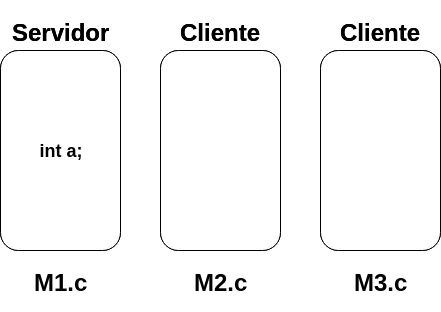
\includegraphics[width=0.5\textwidth]{a.png}
                            \caption*{Ex: int a;}
                        \end{figure}

                  \item Declarações externas contidas no módulo cliente e que somente declaram o nome sem associá-lo a um espaço de dados.

                        \begin{figure}[h]
                            \centering
                            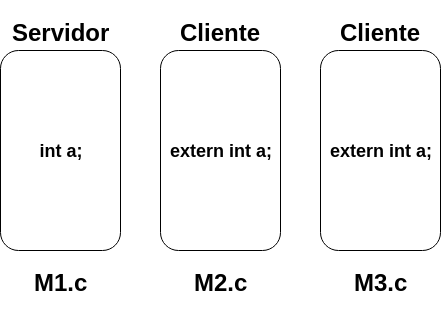
\includegraphics[width=0.5\textwidth]{b.png}
                            \caption*{Ex: extern int a;}
                        \end{figure}

                  \item Declarações e definições de nomes globais encapsulados no módulo.

                        Ex: static int a;

              \end{enumerate}




    \end{enumerate}

\end{doublespace}
%----------------------------------------------------------------------------------------

\end{document}
